\documentclass[12pt,fleqn]{article}\usepackage{../../common}
\begin{document}
Ders 8

İndis Teorisi

Şimdiye kadar yerel metotlarla ilgilendik, mesela lineerizasyon. Lineerizasyon
bir sabit noktanın sonsuz küçük uzaklıktaki çevresine bakıyordu. Kıyasla İndis
Teorisi tüm faz portresine bir bütün şekilde bakabilir ve bu bütün hakkında
bilgi verebilir. 

İndis Teorisi nedir? Ondan önce, indis nedir? Bu arada birazdan göreceğimiz
kavramlar topoloji dersini almış olanlara tanıdık gelebilir. Ya da kompleks
analiz dersi aldıysanız sargılanan sayılar (winding numbers) kavramı ile
alakalar var, ya da artık teorisi (residue theorem) ile bağlantılar
var. Bunların hepsi topolojik kavramlar. Fizikte elektrikte Elektrostatik için
Gauss'un Kanunu'nu hatırlatabilir. 

Kapalı eğri $C$'nin indisi ile başlayalım, $C$ basit bir kapalı eğri, basit
demek kendisiyle kesişmiyor demek. Örnekler altta, soldaki basit sağdaki
değil.

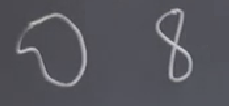
\includegraphics[height=2cm]{08_11.png}

Bu kapalı eğrileri faz uzayının içine koyacağız, ve o vektör alanının eğriden
nasıl dışarı çıktığına bakarak, faz uzayı hakkında bilgi toplamaya
uğraşacağız. Basit kapalı eğrilerin kendisi de bir dinamik sistemin kapalı gidiş
yolu olabilir, ama bu gerekli değil, ve çoğunlukla olmazlar. Ayrıca sabit nokta
içinden geçmeyecek şekilde onları tasarlarız (ama kapalı eğri içindeki bölgede
sabit nokta olabilir).

Kapalı eğrileri elekstrostatikte, ya da sıvı mekaniğindeki Gaussian yüzeyine
benzetebiliriz; onları vektör alanına koyarız, ve bu sayede alanda ne olduğu
anlamaya uğraşırız.

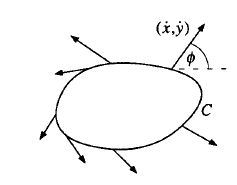
\includegraphics[height=4cm]{08_12.png}

Üstte bir örnek. Bir kapalı eğriyi vektör alanına koyduk, ve o eğri üzerindeki
bir $x,y$ noktasından doğal olarak bir vektör dışarı çıkıyor olacak, bu vektör
$\dot{x},\dot{y}$ ile tanımlı. Bu vektörün açısına bakabiliriz, ona $\phi$
diyelim.

$$ \phi = \tan^{-1} \bigg[ \frac{\dot{y}}{\dot{x}} \bigg] $$

Bizim ilgilendiğimiz eğrinin etrafında saat yönünün tersine doğru bir tur atmak;
bunu yaparken herhangi bir noktadan başlıyoruz ve tüm geçtiğimiz noktalardaki
vektörlerin açısına bakıyoruz, ve bu vektörlerin açılarının değişimini
gözlemliyoruz; sıra halinde bakılınca bu açılar kaç tane tam tur yapmış olurlar?
Üstteki resimlerde eğri üzerinde bazı örnek vektörler gösterilmiş. 

Formel olarak $C$ üzerindeki her $\underline{x}$ noktasında, eğri etrafında saat
yönü tersinde bir kez dönerken $\phi$ sürekli olarak değişir. Eğer
$\dot{x},\dot{y}$ $\underline{x}$'in sürekli bir fonksiyonu ise (ki vektör
alanını hep pürüzsüz olarak farz ettik), o zaman $\phi$ de $\underline{x}$'in
sürekli bir fonksiyonu olacaktır. $[\phi]_C$ bu gidiş sırasında $\phi$'nin net
değişimi [yani tüm değişimlerin toplamı] olsun. O zaman

$$ I_c = \frac{1}{2\phi} [\phi]_C $$

$C$'nin vektör alanı $(\dot{x},\dot{y})$'ye göre indisidir. 

Örnek

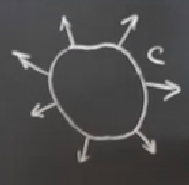
\includegraphics[height=4cm]{08_13.png}

Üstteki gibi bir eğri çizdik, ve herhangi bir noktadan başlayarak (en sağdaki ok
mesela) saat yönü tersine gidiyoruz, ve başladığımız yere dönüyoruz. Bu sırada
açılar tam bir tur atmış olurlar. O zaman $[\phi]_C = 2\pi$, yani $I_C = +1$. 

Eğer hala zihnimizde canlandıramıyorsak, hareket sırasındaki üzerinden geçilen
bazı vektörleri numaralayabiliriz, 

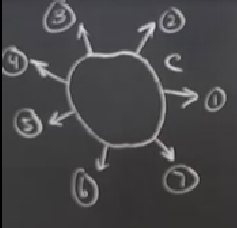
\includegraphics[height=4cm]{08_14.png}

ve onları çıkış noktaları aynı nokta olacak şekilde tekrar çizeriz,

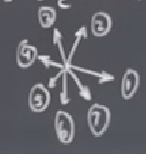
\includegraphics[height=4cm]{08_15.png}

1,2,3 diye giderken tam bir tur atmış olduk.

Soru

İndis kavramının bir vektör alanının curl'ü ile bir bağlantısı var mı?

Cevap

Curl bir vektörün yerel rotasyonu hakkında bize bir şeyler söyler evet, curl ile
indis arasında matematiksel bağlantılar da var, bazı entegral teorileri
üzerinden, ama unutmayalım curl tek bir noktada tanımlıdır, indis ise bir eğri
üzerinde tanımlı, yani indis curl'e göre daha global bir kavram. 

Bir başka örnek görelim şimdi; mesela

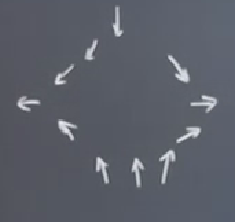
\includegraphics[height=4cm]{08_16.png}

Değişik bir görüntü bu; tüm bu okları kapsayan bir kapalı eğri çizmek kolay
olmayacak ama şöyle bir şekil çizeyim,

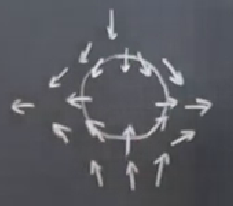
\includegraphics[height=4cm]{08_17.png}

Şimdi parmağımı en sağdaki okla aynı hizaya getireyim, ve saat yönü tersine
giderken parmağımın ne yaptığına bakayım. İlginç bir şey olacak, hareket saat
yönü tersi ama ok yönlerinin gidişatı saat yönünde.

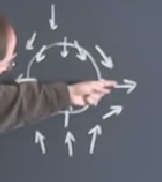
\includegraphics[height=3cm]{08_18.png}
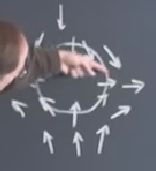
\includegraphics[height=3cm]{08_19.png}
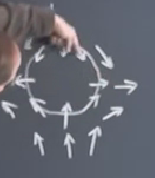
\includegraphics[height=3cm]{08_20.png}
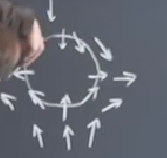
\includegraphics[height=3cm]{08_21.png}
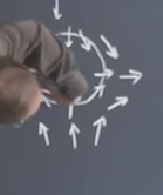
\includegraphics[height=3cm]{08_22.png}

En son karede görüldüğü gibi dönüş açısı elle gösterirken beni şekilden şekilde
soktu ama dönüş yönü hakikaten böyle absürt; eğri üzerinde saat yönü tersi ama
okların dönüşü saat yönünde. 

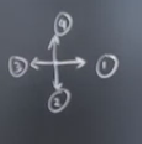
\includegraphics[height=3cm]{08_23.png}

Buradaki indis $I_c = -1$, çünkü dönüş tam tersi yönde. 

Ya alttaki gibi bir akış olsaydı? 

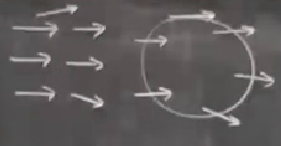
\includegraphics[height=3cm]{08_24.png}

Tam düz sağa doğru akış var, sadece akışın en üstünde ve en altında birer ok
biraz sapmışlar, biri daha üste biri aynı derecede daha alta. Bu akış üzerinde
üstte sağdaki gibi bir eğri çizseydim, ve dönüş sırasında okları takip etseydim,
net dönüşün 0 olduğunu görecektim, $I_c = 0$. 

Başlangıç örnekleri olarak bunlar yeterli herhalde. Şimdi indislerin bazı
matematiksel özelliklerini geliştireceğim, bu özellikler bize dinamik sistem
analizinde yardım edecek şeyler, tek bir indis sayısı hesaplamaktan daha
fazlası var yani.

Özellikler

Ufak bazı teoriler vereceğim şimdi, bazen ispatsız, bazen kaba hatlarla, genel
bir fikir verecek şekilde.

1) Kapalı bir gidiş yolunun indisi: bu teori ``ya kapalı eğrinin kendisi de bir
gidiş yolu ise, ne olur?'' sorusunu soruyor. Yani kapalı eğriyi çiziyoruz ve
vektörlerin hepsi eğriye teğet. 

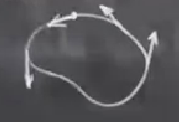
\includegraphics[height=3cm]{08_25.png}

Bu durum eğer eğrinin kendisi de gidiş yolu olsaydı meydana çıkardı. Böyle bir
durumda dönüşte okları takip edersek eğri etrafındaki dönüş sırasında oklar
aynen kapalı eğri gibi tam bir tur atmış olacaktır, ve 1. özellik (ve onunla
ilgili teori) der ki kapalı bir gidiş yolunun indisi her zaman 1
olmalıdır. İspatsız veriyoruz.

Kapalı gidiş yollarıyla ilgileniyoruz çünkü onlar periyotsal hareketleri temsil
ediyorlar.

Soru

-1 sonucunu da elde edebilir miydik?

Cevap

Hayır; kapalı bir gidiş yolu var ise sonuç her zaman +1 olmalı. İspat için
gayrı-Lineer diferansiyel denklemler hakkında  Jordan ve Smith tarafından
yazılmış kitaba bakılabilir, daha fazla referanslar benim kitabımda var.

2) İndislerin eğri $C$'nin parçaları üzerinde toplanır (additive) olabilme
özelliği var.

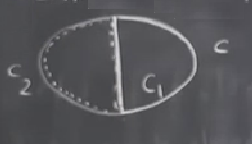
\includegraphics[height=3cm]{08_26.png}

Diyelim ki bir eğri $C$ var. Onu ortasından dik bir çizgi çekerek iki parçaya
bölüyorum, $C_1$ ve $C_2$ (düz çizgi her iki parçaya da ait). Bu eğrilerin
üzerinde yine saat yönü tersine giderek indisi hesaplasaydım, $I_C = I_{C_1} +
I_{C_2}$ olduğunu görürdüm. İspatın ana fikri şöyle, mesela $C_1$'in indisini
hesaplıyorum, ve ortadaki düz bölüm üzerinden geçerken oradaki vektörler
üzerinden $\phi$'deki net değişimi hesaplıyor olacağım, fakat o çizgi üzerinde
net değişim ne ise, $C_2$ için aynı hesabı yaparken $C_1$ hesabı sırasında
gittiğim yönün tam tersine gidiyor olacağım için o net değişimin etkisini
tamamen yoketmiş olurum! Yani toplarken bölen çizgideki hesap iki parça için
birbirini yokeder, geriye sadece eğrilerin indis hesapları kalır. 

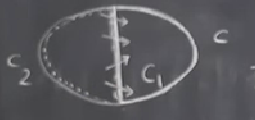
\includegraphics[height=3cm]{08_27.png}

3) Eğer $C$ süreklilik bozulmayacak ve bir sabit nokta içinden geçmeyecek
şekilde yamultulursa (deform), yeni hal $C'$'in indisi $C$ ile aynıdır.

Bu özellik elektrostatikte Gauss'un kanunu hakkında bize bir fikir verebilir
aslında; bir Gaussian yüzey var ve onun içinden olan akıyı (flux)
hesaplıyoruz. Bu durumda Gauss'un kanunundan biliriz ki akı içeride olan yüke
(charge) bağlıdır, yüzeyi yamultuyorum ama bu yamultmayı hiç yük kaybetmeyecek
şekilde yapıyor isem akıyı değiştirmemiş olurum. Benzer durum, eğrinin yerini
değiştirmek indiste değişim yaratmaz.

Bu özelliğin neredeyse tam bir ispatını vereceğim. Pür teorik matematik
derslerinde birazdan göstereceğim türden argümanları çok görürsünüz, çok çekici
şeyler, ve o kadar basitler ki bazen insan şaşırıyor, ispat bu kadar basit mi
diye? Fakat hakikaten ispat bu kadar basit.

İspat

$I_C$'nin $C$'ye sürekli bir şekilde bağlantılı olduğunu biliyoruz. Bu ne demek?
Eğer $C$ üzerinde ufak bir değişim / yamultma yapsaydım, bu sürekli bir şekilde
indis hesabı için baktığım $\phi$'lere yansırdı, çünkü eğrinin üzerinde olduğu
vektör alanı sürekli.

Süreklilikten bahsettik ama $I_C$ bir tamsayı. Bunu nereden biliyoruz? Çünkü
indis hesabı için belli bir yöndeki oku (vektörü) baz alarak başladık, ve
tekrar aynı oka geri döndük. Bu dönüş sırasında eğri üzerinde bir dönüş yaptık,
ve aynı yöne döndüysek ya birkaç kere döndük, ya bir kere döndük, ya da hiç
dönmedik; ama net değişim muhakkak bir dönüşün tamsayılı bir katı olmalı,
kesirsel (reel bir sayıya bağlı) bir kat olamaz, çünkü vektör alanı
süreklidir. O zaman şu sonuca varıyoruz, eğer elimizde tamsayı sonucu olan bir
sürekli fonksiyon var ise bu fonksiyon bir sabit olmalı. Yani $I_C$, ki $C$'nin
bir fonksiyonu, $C$'yi değiştirirken sabit kalmalı, $I_C = I_{C'}$.

Tamsayı değerli fonksiyonları yamultma üzerinden görsel örnekte görelim;

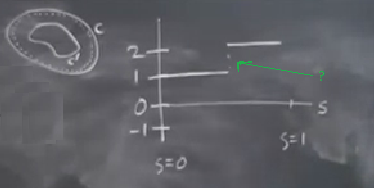
\includegraphics[height=4cm]{08_28.png}

Diyelim ki $S$ parametresi $C$'yi ne kadar yamulttuğumuzu kontrol ediyor, $x$
ekseninde sağa gittikçe o oranda $C$'yi yamultmuş oluyoruz (resimde soldaki
eğri). Ve diyelim ki yamulta yamulta $S=1$'e geldik, o noktada büyük $C$ onun
içindeki $C'$ haline geldi. Bunun yansıması resimde sağdaki grafik üzerinde neye
benzer? Yamultma olurken tamsayı 1 seviyesindeyiz, sonra... bir noktada 2
olabilir miyiz? Bunun için bir ``zıplama'' gerekir, ama bu zıplama bir
fonksiyonun sürekliliğine aykırıdır. Bu kadar. Bu da olamayacağına göre tam sayı
çıktılı bir sürekli fonksiyonun varlığı bu fonksiyonun sabit olduğu anlamına
gelir.

Bu arada yamultma sırasında sabit nokta içinden geçmeme şartını nasıl kullandık?
Bu şarta uyulmalı çünkü tam sabit nokta üzerinde üzerinden $\phi$
hesaplayacağımız vektör nedir? Sıfırdır. Bu tür durumlarda indis tanımlı
olamayacağı için sabit noktalara girmiyoruz.

4) Diyelim ki $C$ içinde hiç sabit nokta yok. Bu durumda $I_C = 0$
olmalıdır.

İspat için bir $C$'yi düşünelim, onu küçülte küçülte tek bir nokta seviyesine
getiriyorum, o anda $C$'den çıkan vektörlerin hepsi aynı yönü gösteriyor
olmalılar, bunu vektör alanının sürekliliğinden biliyorum. Ufacık bir kapalı
eğri içinde vektörlerin tam bir dönüş yapma şansı yoktur, o zaman içinde sabit
nokta olmayan ufacık bir $C'$ için $I_{C'} = 0$ olmalı, o zaman, biraz önce
gördüğümüz 3. özellik yüzünden $I_C$ de sıfır olmalı.

5) İndisin bize sabit noktaların stabilitesi hakkında bilgi verebileceği
düşünülebilir, fakat bu doğru değil, arada hiç bağlantı yok. Daha formel şekilde
tarif edelim; diyelim ki zamanı tersine çevirdik, $t \to -t$ oldu, vektör
alanındaki tüm oklar 180 derece tersine döndü (ya da $\dot{\underline{x}} \to
-\dot{\underline{x}}$ oldu). Bu demektir ki her noktada $\phi$ eklenir, $\phi \to
\phi + \pi$ olur, ama bu ekleme $[\phi]_C$'de, yani $\phi$'nin net değişimi
üzerinde hiçbir etki yaratmaz, çünkü her şeye $\pi$ ekledim, bu ekler net
değişim hesaplanırken iptal olacaktır. Demek ki zamanı tersine çevirmek indisi
etkilemez.

Sabit noktanın stabilitesi hakkında bilgi alamayız, eğer zamanı tersine
çevirseydim eğri içindeki stabil nokta gayrı-stabil hale gelirdi, ama bu durum
indisi etkilemezdi, evet, indisler sabit nokta stabilitesi hakkında bir şey
söylemez, ama sabit noktaların {\em türü} hakkında birşeyler
söyleyebilir. Mesela düğüm (node) sabit noktasının indisi her zaman +1, eyer
(saddle) düğümünün indisi her zaman -1'dir (düğümün stabil mi gayrı stabil mi
olduğu fark etmiyor, 5. özellik yüzünden).

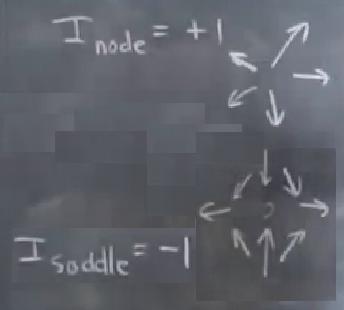
\includegraphics[height=5cm]{08_29.png}

Devam edersek, sarmal (spiral) için +1, merkez (center) için yine +1.

Sabit nokta olmayan herhangi bir nokta için indis her zaman sıfırdır. Çünkü o
noktanın içinden vektörler sadece geçip gidiyor olabilirler, bu durumda, sadece
tek bir yöne gidildiği bir durum var, indis sıfır.

Tüm bunları hatırlamak için daha önce lineerizasyonda kullandığımız iz,
determinant diyagramları faydalı olabilir. 

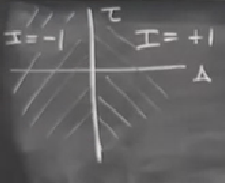
\includegraphics[height=4cm]{08_30.png}

Sağ bölgede indis her zaman 1, merkezler, düğümler, sarmallar orada
yaşıyor. Sol bölgede indis her zaman -1, eyerler burada. Tam yatay eksen
üzerinde, hatırlarsak, lineerizasyonda izole olmayan sabit noktalar vardı, bu
bölgede indis hesaplanamıyor, çünkü elimizde izole olan sabit nokta yok, bu
sebeple sadece o noktayı kapsayacak şekilde bir kapalı eğri çizmemiz mümkün
değil, yani indis hesaplamamız mümkün değil.

Soru

2'den büyük ya da -2'den küçük indis değerine sahip bir sabit nokta olabilir
mi?

Cevap

Şimdiye kadar gördüğümüz sabit nokta sınıflamaları için değil ama, evet, bu
değerleri verebilecek tür sabit noktalar var. Mesela dinamik sistem $\dot{x} =
z^n$, ki $z = x + iy$, yani kompleks bir sayı var, ve bu sistemin vektör alanına
bakarsak böyle durumları görebiliriz, mesela $\dot{z} = z^2$, o zaman $\dot{x} +
i\dot{y} = x^2 + y^2 + i(2xy)$. Buna tekabül eden vektör alanı,

$$ \dot{x} = x^2 - y^2 $$

$$ \dot{y} = 2xy $$

Bu sistemin lineerizasyonu tamamı sıfır olan bir matris olurdu, lineerizasyonun
hiçbir şeyden haberi yok, sistemi orijinde zannediyor ve orada sabit noktalardan
oluşan bir düzlem var zannediyor. Fakat bu doğru değil. Orijinde tek bir sabit
nokta var, vektör alanına baksak ve indis hesaplasak değeri +2 (ya da -2, tam
hatırlayamıyorum, ama ikisinden biri).

Ya da bir diğer örnek, fizikte ikili kutup (dipole) problemleriyle uğraşanlar bu
tür sistemleri görürler, mesela vektör alanı şöyle ise,

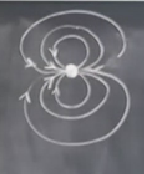
\includegraphics[height=4cm]{08_31.png}

indis değeri 2 çıkar (ya da -2). Üstteki türden bir dinamik sistem bu derste
görmedik ama tabii ki böyle sistemler var. 

Neyse devam edelim,

Teori

$\mathbb{R}^2$'deki her kapalı gidiş yolunun içinde muhakkak sabit nokta(lar)
vardır, ve bu noktaların indisinin toplamı +1 olmalıdır, $\sum_{k=1}^{n} I_k =
1$.

Belki bazılarınız böyle bir sonuç çıkabileceğini tahmin etmiştir; mesela iki
kuyulu titreşiri düşünürsek,

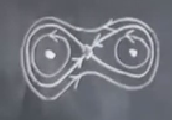
\includegraphics[height=4cm]{08_32.png}

Sağda ve solda merkez, tam ortada eyer düğümü vardı, indisler sağda solda +1,
ve ortada bir -1.

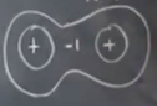
\includegraphics[height=2cm]{08_33.png}

Eğer en dıştaki kapalı gidiş yolunu düşünürsek ve ona göre indis hesaplarsak
içeride +1, +1 ve -1 var, toplam +1. Ve bu kapalı gidiş yolunun indisi
hakikaten +1. Peki nasıl böyle oldu? 3. özellik yüzünden. Eğer kapalı eğriyi üç
parçaya bölsek, 

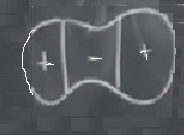
\includegraphics[height=3cm]{08_34.png}

Tüm eğri indisi için o parçaları toplayabilirdik, ve üstteki örnek için +1
değerini elde ederdik.

Bu çok güzel bir teori çünkü kapalı bir gidiş yolu içinde neler olabileceğine
kısıtlamalar getiriyor (ve bizim analizlerimize kolaylaştırma sağlıyor). Bu
teorinin güzel bir diğer tarafı, mesela bazen elimizde bir dinamik sistem oluyor
ve düşünüyoruz ki bu problemde kapalı gidiş yolları yok, ama emin değiliz, ve
biraz önce gördüğümüz türden argümanları kullanarak kapalı gidiş yolu varlığını
hemen devre dışı bırakabiliyoruz.

Örnek

Tavşan vs koyun problemine dönelim;

$$ \dot{x} = x(3 - x - 2y) $$

$$ \dot{y} = y(2-x-y) $$


Ortada bir eyer düğümü vardı, eksenlerde düğümler, orijinde gayrı stabil
düğüm. Peki bu resimde nasıl kapalı bir yörünge ortaya çıkardı? 

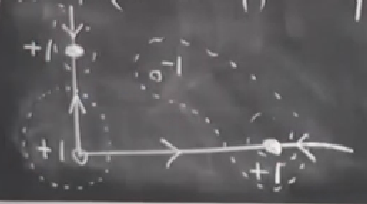
\includegraphics[height=4cm]{08_35.png}

Üstteki görülen noktalı çizgiyle gösterdiklerimizin hiçbiri mümkün değil; orijin
etrafındaki olmaz çünkü gidiş yolları kesişemez. Sağdaki iki sabit noktayı
kapsayan olmaz çünkü indis toplamı sıfır (+1 olmalıydı). Sol üstteki, aynı
şekilde, gidiş yolu kesişmesi. Sadece ortadaki nokta etrafındaki de olmaz, orada
indis -1 değerinde. Herhalde ana fikri anlatabiliyorum, bu problemde kapalı
yörünge yok, ve bunu indis teorisini kullanarak hemen anladık. 

Soru

Kapalı bir yörünge içinde hiç sabit nokta olmaması mümkün değil mi?

Cevap

Hayır. Daha önce demiştik ki 1. özelliğe göre kapalı gidiş yollarının indisi +1
olmalı. O zaman içerideki sabit noktaların indisinin toplamı +1 olmalı, eğer
içeride hiç sabit nokta yoksa, sabit nokta olmayan noktaların indisi sıfır
olduğu için toplam da sıfır olurdu, ve bu kapalı gidiş yolunun indisinin 1 olma
kuralına ters düşerdi. 

Bu noktada İndis Teorisi hakkında söyleceklerim bitti. 

Bir sonraki bölüme atlıyoruz şimdi; 7. bölüm.

Limit Çevrimleri (Limit Cycles)

Bunlar çok önemli izole, kapalı gidiş yolları. İzole derken limit çevrimlerin
yanındaki gidiş yolları kapalı değil demek istiyorum. Yani mesela merkezlerden
farklı olarak, ki bu durumda faz portrelerinde merkez yakında pek çok çeşit
kapalı eğri oluyordu, bir dış gidiş yolu içinde bir sarmal olabiliyor,

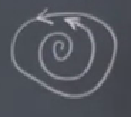
\includegraphics[height=4cm]{08_36.png}

Üstteki gibi. ``Limit'' kelimesinin nereden geldiği görülüyor herhalde, üstteki
resimde dışarıdaki eğri içerideki sarmal için bir tür ``limit''. Sonuşurda
(asymptotically) ona yaklaşıyor. Tipik olarak dışarıda bir tane daha eğri olur,
o da limit çevrimine yaklaşır,

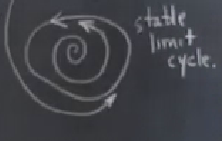
\includegraphics[height=4cm]{08_37.png}

Bu duruma ``yaklaşılan'' şeye stabil limit çevrimi (stabil limit cycle) ismi
veriliyor. Gayri stabil olanları da var,  

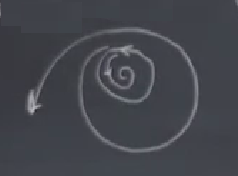
\includegraphics[height=4cm]{08_38.png}

Bu durumda ortadaki limit çevrimi dışındaki gidiş yolu ondan uzaklaşıyor.

Nadir de olsa marazi (pathalogical) durumlar oluyor tabii, yarı stabil limit
çevrimler, dışarıdan gayrı stabil içeriden stabil.

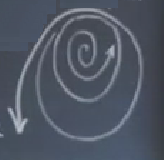
\includegraphics[height=4cm]{08_39.png}

Peki limit çevrimleriyle niye ilgileniyoruz? Onlar, mesela stabil limit
çevrimleri, sistemin yapmak istediği periyotsal bir gidişi temsil ediyor, yani
pek çok farklı başlangıç konumundan o çevrime doğru bir yöneliş / çekim
var. Eğer sistem bir tür kalıcı salınıma doğru meyil ediyorsa, büyük bir
ihtimalle o sistemin arka planda stabil bir limit çevrimi vardır. 

Pek çok farklı bilim alanında limit çevrimleri ortaya çıkar; biyolojide mesela
kalbin çarpması ve onu kontrol eden biyoelektrik sistemi bir limit çevrimine
göre ayarlıdır. Ya da gün içinde aşağı ve yukarı inen çıkan vücut ısımız limit
çevrimine bağlıdır. Mühendislikte kontrol sistemlerindeki geribesleme bir diğer
örnek, isteniyorlarsa iyi tabii ama bazen istenmeyen şekilde ortaya çıkıyorlar,
mesela uçakta giderken kanatlara bakın, bir titreme varsa uçak
spesifikasyonlarının belirttiğinden daha hızlı uçurulduğunda aşağı yukarı
hareket ederler. Bunu yapmamaları gerekir, uçak uçaktır, kuş değil, kanatlarını
çırpmasına gerek yok.

Ya da köprülerin sallanması. Ya da pencere güneşlikleri; aralarından tutarlı bir
hızda bir rüzgar esiyor ve bakıyorsunuz güneşlik takırdamaya başlıyor. Sabit bir
güç etki ediyor, yani periyotsal bir etki yok, sabit etki var, ama birdenbire
güneşlik salınıma giriyor. Pek çok örnek.

Son bir nokta: lineer sistemlerde limit çevrimleri olmaz, çünkü limit
çevrimlerinin özü gayrı lineer. Lineer sistem derken ben bu terimi başkalarından
biraz farklı kullanıyorum, $\dot{\underline{x}} = A \underline{x}$, ki
$A$ içinde sabit katsayılar olan bir matris. Bu tür bir sistem var ise orada
limit çevrimi olamaz. Kapalı yörünge olabilir, ama bu yörüngeler izole
olmayacaktır. Bu tür sistemlerde periyotsal çözümler izole olmaz. Eğer $x(t)$
periyotsal bir çözüm ise $c x(t)$ de periyotsal bir çözümdür.

Yani elimde bir çözüm varsa (alttaki resimde en içerideki kapalı eğri), 

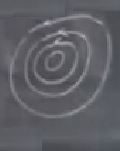
\includegraphics[height=4cm]{08_40.png}

o zaman o çözümü bir sabitle çarparak / ölçekleyerek bir sürü diğer çözümleri de
elde edebilirim (tüm dış kapalı eğriler).

Üstteki durum limit çevrimi değil, çünkü sistemdeki ufak bir gürültü bizi bir
eğriden diğerine atabilir, ve sistem sonsuza kadar o yolda kalacaktır. Fakat
limit çevriminde eğer bir düzenini bozma durumu (disturb) var ise tekrar geri
dönersiniz. Yani bu tür sistemler daha sağlamdır (robust).

Ödevler

Soru 3.1.3

Alttaki ödev sorusu için niteliksel olarak farklı olan tüm vektör alanlarını
$r$'nin değişimi üzerinden taslaksal olarak çizin. Başta ne olduğunu
bilmediğimiz kritik bir $r$ değerinde eyer düğümü çatallaşması olduğunu
gösterin. Ve en son olarak çatallaşma diyagramını $x^\ast$ ve $r$'li olacak şekilde
taslaksal çizin.

$$ \dot{x} = r + x - \ln(1+x) $$

Cevap

Her ne kadar $\dot{x}=0$'i çözmek problemli olsa da, $r$ için çözmek
$r=\ln(1+x)+x$ sonucunu veriyor. $\ln(1+x)$ formülü $x \ge 1$ değerleri
üzerinden tanımlı olabilir sadece. $x \to -1$ ya da $x \to \infty$ olduğu
durumda $r \to -\infty$ olur. O zaman $r>0$ için hiçbir sabit nokta
yoktur. $r<0$ için $x=-1$'e yaklaşan sabit nokta stabildir, diğeri gayrı
stabildir.

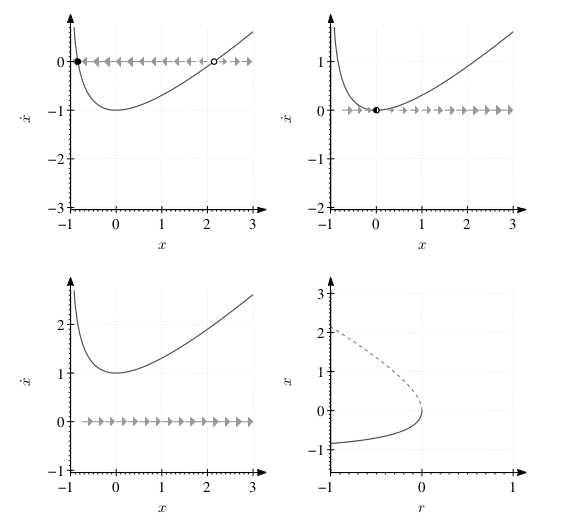
\includegraphics[height=12cm]{08_01.png}

Üstteki grafiklerde sağ alttaki hariç tüm diğerleri $\dot{x} = r+x-\ln(1+x)$'in
faz uzayı. Üst solda $r=-1$, üst sağda $r=0$, alt solda $r=1$, alt sağda
$\dot{x} = r+x-\ln(1+x)$'in çatallaşma diyagramı. 

Soru 3.2.2

Alttaki soru için $r$ değiştikçe ortaya çıkacak tüm niteliksel olarak farklı
vektör alanlarını taslaksal olarak çizin. Kritik bir $r$ değerinde transkritik
çatasllaşma olduğunu gösterin. Çatallaşma diyagramını $x^\ast$ ve $r$'li olacak şekilde
taslaksal çizin.

$$ \dot{x} = rx - \ln(1+x) $$

Cevap

Burada bir sabit nokta $x_1=0$ üzerinde hareket ediyor, ve bu nokta $r<1$ iken
stabil. Ama $r=1$ olunca $x=\infty$'da ikinci bir sabit nokta ortaya çıkıyor,
$r=1$'de gayrı stabilden stabile dönüşüyor. Bu noktada $\dot{x}$ $x=f(r)$'e
transform edilemez, bu sebeple olanları tarif etmek için $r =\frac{\ln(1+x)}{x}$
kullanıldı. $r\to\infty$ iken stabil nokta $x=-1$'e yaklaşır.


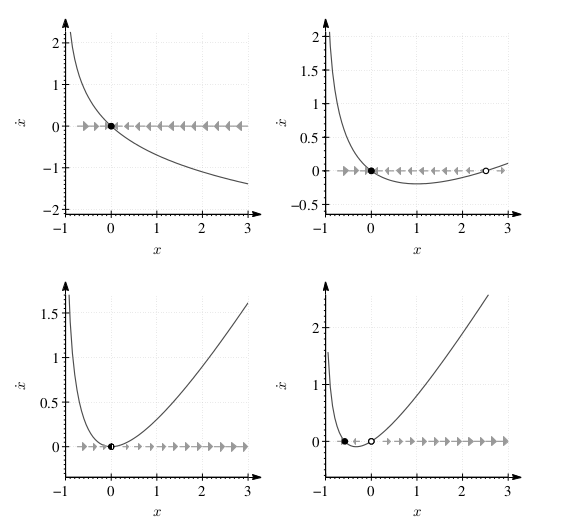
\includegraphics[height=12cm]{08_02.png}

Üsttekiler faz uzayıdır. Sol üst $r=0$, sağ üst $r=0.5$, sol alt $r=1$, sağ alt
$r=1.5$.

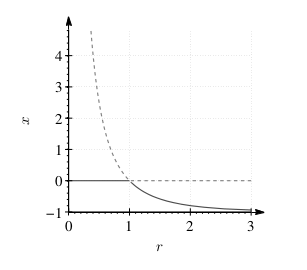
\includegraphics[height=6cm]{08_03.png}

Üstteki ana formülün çatallaşma diyagramı.

Soru 3.4.6

Bu soru farklı çatallaşmalar arasındaki farkı görebilmeniz için hazırlandı,
çünkü farklı tipleri birbirine karıştırmak çok kolay! Alttaki soruda hangi $r$
değerinde çatallaşma olduğunu bulun, ve eğer mi, transkritik mi, süperkritik
tırmık mı, yoksa altkritik tırmık mı bunu bulun. Son olarak çatallaşma
diyagramını $x^\ast$ ve $r$'li olacak şekilde taslaksal çizin.

$$ \dot{x} = rx - \frac{x}{1+x} $$

Denklemi faktorize edince sabit noktaların, $r \ne 0$ olduğu zaman, $x^\ast=0$ ve
$x^\ast=(1/r)-1$ üzerinde olacağını görmek oldukça kolay. Alttaki $x^\ast,r$ bazlı
çizilen figürde

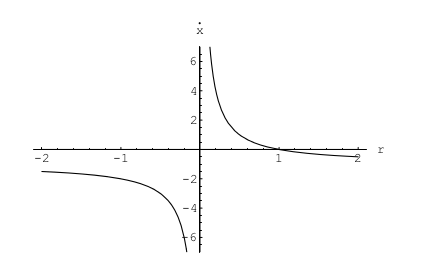
\includegraphics[height=6cm]{08_04.png}

bir transkritik çatallaşma olduğunu görüyoruz. Kontrol etmek için eğer
$\dot{x}=f(x)$ ise $f'(x) = r - (1+x)^2$ olduğuna dikkat edelim. $x^\ast=0$ olduğu
zaman önceki ifade $f'(x) = r-1$'e dönüşür. Bunun anlamı sabit noktanın $r<1$
niçin gayrı stabillikten $r>1$ için stabilliğe doğru değişeceğidir (türevin o
noktadaki işaretinden bunu anlayabiliyoruz). Bu demektir ki $r_c = 1$ noktasında
bir transkritik çatallaşma var. Diyagramı altta.

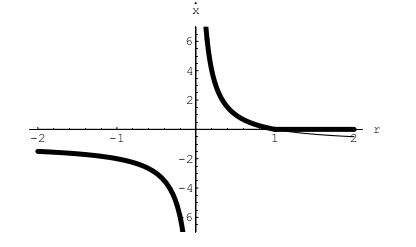
\includegraphics[height=6cm]{08_05.png}

Soru 3.4.14

$\dot{x} = rx + x^3 - x^5$ sistemini düşünelim ki bu sistem altkritik tırmık
çatallaşmasına sahip.

a) $r$ değişirken ortaya çıkacak tüm sabit noktaların cebirsel ifadesini bulun.

b) $r$ değişirken ortaya çıkan vektör alanlarını taslaksal çizin. Tüm sabit
noktaları ve onların stabilitesini göstermeyi unutmayın.

c) Eyer düğümü çatallaşması sırasında sıfır olmayan sabit noktaların doğduğu
$r_s$ noktasını hesaplayın.

Cevap

a) Sabit noktalar $x^\ast=0$, ve  $r + x^2 - x^4$'ün çözümleri

$$ x^\ast = \pm \sqrt{ \frac{1}{2} \pm \sqrt{r + \frac{1}{4}} }  $$

Dört tane mümkün işaret $\pm/\pm$ seçimi için dört tane basit olmayan sabit
nokta var. $r<-1/4$ olduğu zaman bu dört noktanın hiçbiri mevcut değil, hepsi
$r=-/14$ noktasındaki eyer düğümü çatallaşması sırasında yaratılıyorlar. 

b)

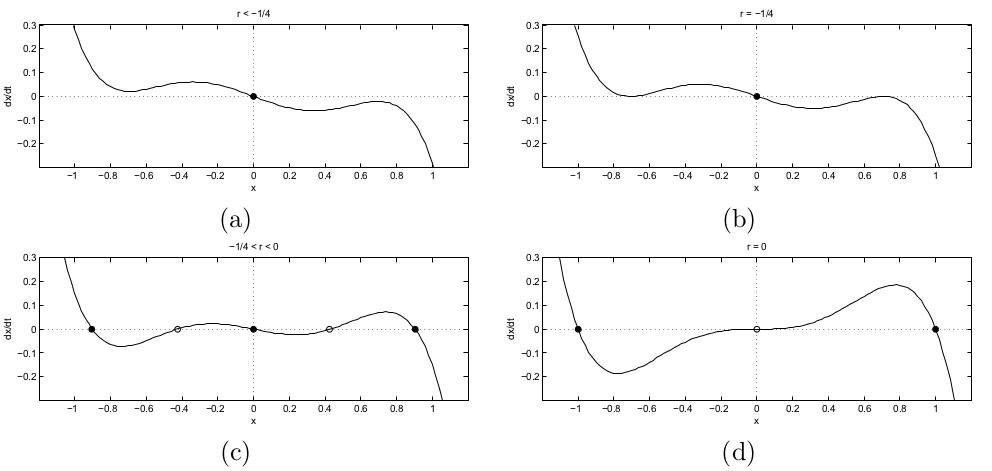
\includegraphics[height=8cm]{08_06.png}

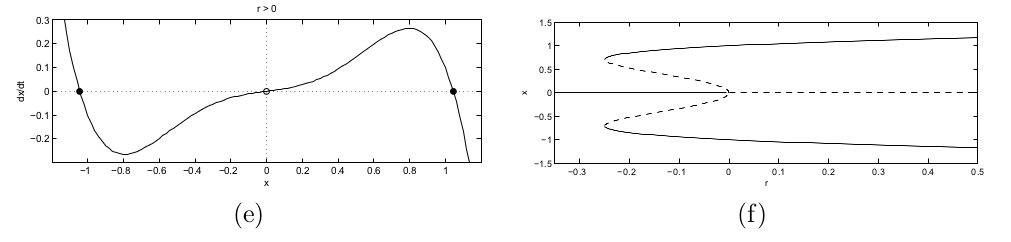
\includegraphics[height=4cm]{08_07.png}

(a) figüründe $r<-1/4$ için tek stabil nokta. (b) $r=-1/4$'te eyer düğüm
çatallaşması, $x=0$ stabil, ortaya yeni çıkan $x - \pm 1/\sqrt{2}$ noktaları
yarı-stabil. (c) $-1/4 < r < 0$ (d) $r=0$'da altkritik tırmık çatallaşması. (e)
$r>0$ için bir gayrı stabil bir stabil sabit nokta. (f) altkritik tırmık
çatallaşması için çatallaşma diyagramı, ki $r=-1/4$'te eyer düğümü çatallaşması
var, ve $r=0$'da tırmık çatallaşması var. Kesiksiz çizgi stabil dalları, kesikli
olan gayrı stabil dalları temsil ediyor. 

c) a) cevabında basit olmayan sabit noktaların formülünde görüldüğü üzere
(ikili) eyer düğümü çatallaşması $r=-1/4$'te. Ya da dinamik sistemi şu şekilde
yazarsak,

$$ \dot{x} = rx + x^3 - x^5 = x \bigg( (r+\frac{1}{4}) - (x^2 - \frac{1}{2})^2  \bigg) $$

bu formülde bariz olarak görülüyor ki sabit noktalar $r=-1/4$ olduğu zaman
$x = \pm 1/\sqrt{2}$'de doğuyor. 

Soru 3.7.5

Zebraların şeritleri ve kelebeklerin kanatlarındaki şekiller biyolojik
şekillerin, kalıpların oluşmasının en müthiş iki örneği. Bu kalıpların nasıl
oluştuğunu açıklayabilmek biyolojinin çözülmeyi bekleyen en büyük
problemlerinden, bilimcilerin şu ana kadar bildiklerini [1] çok güzel
anlatıyor. [2] araştırmasında Lewis ve arkadaşları bu kalıbın oluşmasındaki
öğelerden birini bir biyolojik subap olarak düşündü, biyokimyasal sinyal maddesi
$S$ bir gen $G$'yi aktive ediyordu. Modellerine göre gen normal olarak etkin
olmayan (inactive) bir halde olabilir, ama $S$'in konstrasyonu belli bir
seviyeyi aştıktan sonra bir pigment ya da gen ürünü üzerinden aktif hale
getirilir. $g(t)$ bu gen ürününün konstrasyonu olsun, ve $S$'in konstrasyonu
$s_0$ seviyesinde sabitlenmiş. Model şöyle,

$$ \dot{g} = k_1s_0 - k_2g + \frac{k_3 g^2}{k_4^2 + g^2} $$

$k$'ler pozitif değerli sabitler. $g$'nin üretilmesi $k_1$ hızında $s_0$
tarafından tetiklenir, ve aynı $g$'nin üzerinde $k_2$ oranı üzerinden bir azalış
ta mevcuttur. Bu azalış bir otokatalitik (autocatalytic), ya da pozitif bir
geribildirim (feedback) süreci üzerinden olmaktadır, modelde gayrı lineer terim
üzerinden gösterilir.

a) Sistemin boyutsuz bir forma geçirebileceğini göster, alttaki gibi

$$ \frac{dx}{d\tau} = s - rx  + \frac{x^2}{1+x^2} $$

b) Eğer $s=0$ ise $r<r_c$ için iki tane pozitif sabit nokta $x^\ast$ olduğunu
göster ($r_c$ sonradan hesaplanacak).

c) Farz et ki başta hiç gen ürünü yok, yani $g(0) = 0 $, ve yine farz et ki $s$
yavaş yavaş sıfırdan arttırılıyor (aktivasyon sinyali açılmış). $g(t)$'ye ne
olur? $s$ tekrar sıfıra döndürülürse ne olur? Gen kapatılmış konuma geri mi
döner?

d) Çatallaşma eğrileri için $(r,s)$ uzayında parametrik formülleri bul, ve
ortaya çıkacak çatallaşmaları sınıfla.

e) Bilgisayarı kullanarak sayısal olarak doğru $(r,s)$ uzayında olan stabilite
diyagramını grafikle.

Konu hakkında daha fazla detay [1,2,3]'te bulunabilir.

Cevap

a) 

$x=\frac{g}{G}$, $\tau=\frac{t}{T}$ olsun, o zaman $\frac{dg}{dx} = G$, ve
$\frac{d\tau}{dt} = \frac{1}{T}$ olacaktır. Bu demektir ki,

$$ \frac{dg}{dt} = \frac{dg}{dx}\frac{dx}{d\tau}\frac{d\tau}{dt} =
\frac{G}{T}\frac{dx}{d\tau}
$$

Eğer ana diferansiyel denklemimize dönersek, bu denklem alttaki halde tekrar
yazılabilir,

$$ \frac{dx}{d\tau} = \frac{Tk_1s_0}{G}-\frac{Tk_2}{G}(Gx) +
\frac{T}{G} \frac{k_3(Gx)^2}{k_4^2 + (Gx)^2}
$$

$$ = s - rx + \frac{k_3T}{G} \frac{x^2}{(\frac{k_4}{G})^2 + x^2} $$

ki $s = \frac{Tk_1s_0}{G}$ ve $r = Tk_2$'dir.

Biz $\frac{k_3T}{G} = 1$ ve $\frac{k_4}{G} = 1$ olsun istiyoruz ki $G=k_4$ ve $T
= \frac{k_4}{k_3}$ olsun. Ayrıca

$$ s = \frac{k_4}{k_3}\frac{k_1s_0}{k_3} = \frac{k_1s_0}{k_3}$$

ve

$$ r = \frac{k_4}{k_3}k_2 = \frac{k_2k_4}{k_3} $$

Ve nihayet diferansiyel denklemi şu şekilde tekrar yazıyoruz,

$$ \frac{dx}{d\tau} = s - rx + \frac{x^2}{1+x^2}$$

b) $s=0$ oldugunda

$$ \frac{dx}{d\tau} = - rx + \frac{x^2}{1+x^2}$$

formülü sabit noktaları verir. Açık bir şekilde görülüyor ki bu formülün
$x=0$'da bir çözümü vardır, ve tüm formülü $x$'e böleriz, böylece bu çözümü
unutmayacağımızı garanti etmiş oluruz. Sonuç denklem $rx^2 - x + r = 0 $ olarak
yazılabilir. Bu denklem ünlü karesel formül ile çözülebilir,

$$ x = \frac{1 \pm \sqrt{1-4r^2}}{2r} $$

Bu formül bize $r<1/2$ için iki tane reel ve pozitif kök verecektir. 

c)

Alttaki figürden görülebileceği üzere $r<1/2$ için sadece bir tane stabil sabit
nokta olduğunu buluyoruz. Grafik birkaç farklı $s$ için $x-s$ ile $x^2/1+x^2$
üzerinden basıldı.

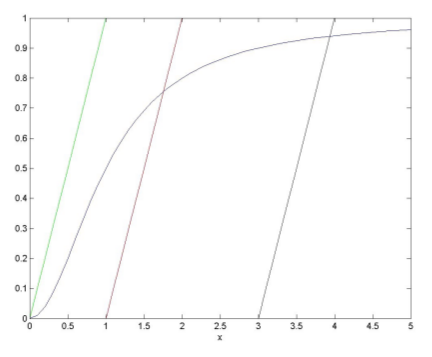
\includegraphics[height=7cm]{08_08.png}

Fakat, ufak $s$ ve $r<1/2$ için 3 tane sabit nokta olduğunu buluyoruz. Bir
tanesi sigmoid'in alt ucuna doğru ve stabil, öteki sigmoid'in ortalarına doğru
ve gayrı stabil, üçüncüsü ise sigmoid'in üst sağ yarımında ve stabil. $s$
arttırıldıkça ilk iki sabit nokta biraraya geliyorlar ve birbirlerini
yokediyorlar, geriye sadece üçüncü kalıyor. Bu davranış alttaki grafikte,

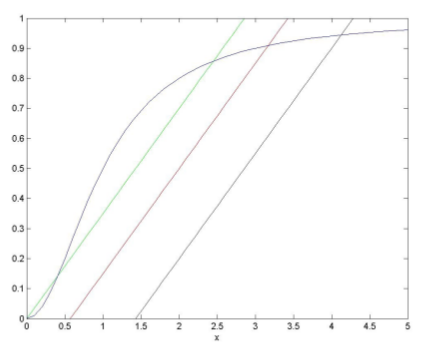
\includegraphics[height=7cm]{08_09.png}

Yani $r>1/2$ için $s$ değiştikçe gen seviyelerinin yukarı aşağı çıkıp inmesini
bekleriz. Fakat $r<1/2$ için $s$ arttıkça gen seviyeleri de artacak. Gen
seviyesinin eğri üzerinde ne kadar üstte olduğuna bağlı olarak $s$ azalırken bu
seviye ya gayrı stabil noktanın altında ya da üstünde takılı kalacak. Yani
sinyalleme maddesi olmasa bile gen üretimi aktif edilmiş halde kalır. 

d)

Eyer düğümü çatallaşmaları $f(x)=0$ ve $f'(x)=0$ iken ortaya çıkar.

$$ \frac{dx}{d\tau} = s - rx + \frac{x^2}{1+x^2}=0 $$

ve

$$ \frac{d^2x}{dxd\tau} = - r + \frac{(1+x^2)2x-x^2(2x)}{(1+x^2)^2} = 0$$

için alttakiler olur,

$$ rx - s = \frac{x^2}{1+x^2} $$

$$ r = \frac{(1+x^2)2x-x^2(2x)}{(1+x^2)^2} = \frac{2x}{(1+x^2)^2}$$

Bunları ana formüle geri sokup $s$ için çözersek,

$$ s = rx - \frac{x^2}{1+x^2} = \frac{x^2-x^4}{(1+x^2)^2} $$

Özet olarak

$$ r_c = \frac{2x}{(1+x^2)^2} $$

ve

$$ s_c = \frac{x^2-x^4}{(1+x^2)^2} $$

e)

Üstteki iki fonksiyonu $x$ parametresi üzerinden grafiklersek,

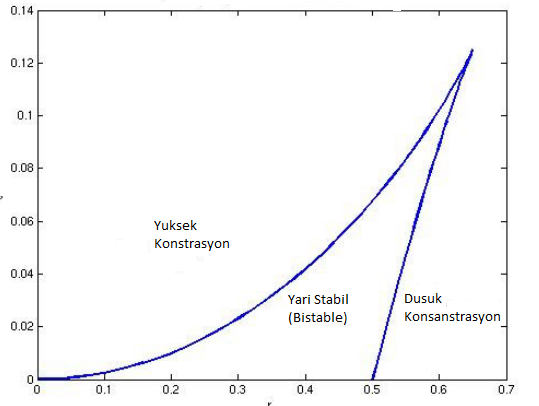
\includegraphics[height=6cm]{08_10.png}

Grafikte biyokimyasal aç / kapa düğmesinin hangi bölgelerde açık ve gen
üretiminin yüksek konsantrasyonda olduğunu, nerede açık / kapalı pozisyonlar
arasında gidip geldiğini, ve düğmenin nerede kapalı ve gen ürününün
konstrasyonunun düşük olduğunu görüyoruz. 

Kaynaklar

[1] Murray, {\em Mathematical Biology}, 1989

[2] Lewis, Slack, Wolpert, {\em Thresholds in development}, Theor. Biol. 65,
sf. 579, 1977

[3] Edelstein-Keshet, {\em Mathematical Models in Biology}

\end{document}



